\documentclass[tc, manuscript]{copernicus}

\setcounter{figure}{0}
\makeatletter 
\renewcommand{\thefigure}{S\arabic{figure}}

\begin{document}

\title{Supporting Information for ``Ice-shelf ocean boundary layer dynamics from large-eddy simulations"}

\runningtitle{IOBL dynamics}

\runningauthor{Begeman et al.}

\correspondence{Carolyn Begeman (cbegeman@lanl.gov)}

\Author[1]{Carolyn Branecky}{Begeman}
\Author[1]{Xylar}{Asay-Davis}
\Author[1]{Luke}{Van Roekel}

\affil[1]{Los Alamos National Laboratory, P.O. Box 1663, Los Alamos, New Mexico, USA 87545}

\firstpage{1}

\maketitle

\noindent\textbf{Contents of this file}

\noindent
Table S1. Parameter choices for simulations.\\
Figure S1. Results of the atmospheric stable boundary layer test case.
Figure S1. Vertical profiles of resolved and sub-grid vertical heat fluxes.\\
Figure S2. Vertical profiles of TKE budget terms for thermal driving simulations.\\
Figure S3. Vertical profiles of the ratio of vertical to horizontal variance.\\
Figure S4. Vertical profiles of sub-grid vertical diffusivities.\\
Figure S5. Vertical profiles of the total vertical salt flux.\\
Figure S6. Vertical profiles of the vertical eddy viscosity.\\
Figure S7. Relationship between thermal driving and melt rate over multiple inertial periods. 

\clearpage

\begin{table*}[t]
\caption{Parameters relevant to the configuration of referenced simulations. Asterisks denote variables whose values were varied between simulations.}
\label{table:var}
\begin{tabular}{column = lcr}
\tophline
Variable & Description & Value\\
\middlehline
$c_d$       & drag coefficient          & 0.003 \\
$c_p$       & heat capacity of water    & 4218\\   
$dP/dx,dP/dy$   & horizontal pressure gradient & $0.0,0.03$ Pa m$^{-1}$\\
$dS/dz$     & far-field vertical salinity gradient & 0.5 PSU km$^{-1}$\\
$d\theta/dz$& far-field vertical temperature gradient & 0.1 $^{\circ}$C km$^{-1}$\\
$h_x,h_y$   & domain width              & 64 m\\
$h_z$       & domain height             & 64 m\\ 
$L_f$       & latent heat of fusion     & $3.3 \times 10^5$ J kg\textsuperscript{-1}\\
$P_0$       & domain top pressure       & 800 dbar\\
$Pr$        & Prandtl number            & 13.8\\
$rdf$       & Rayleigh damping coefficient & 0.0001\\
$S_{\infty}$& far-field salinity        & $35$ PSU \\
$Sc$        & Schmidt number            & 2432\\
$\alpha$    & *ice shelf slope          &$0.01$ to $1.0^{\circ}$ \\
$\beta$     & angle between vector oriented up-slope and North & 90$^{\circ}$\\
$\beta_m$   & Businger coefficient for momentum & $-4.8$ \\
$\beta_{\theta}$& Businger coefficient for temperature & $-5.6$ \\
$\beta_S$   & Businger coefficient for salinity & $-5.6$\\
$\Delta_x,\Delta_y$& horizontal resolution  & 0.5 m\\
$\Delta_z$  & vertical resolution       & 0.25 m\\
$\Gamma_{\theta,mol}$& thermal molecular exchange coefficient  & $12.5 \textrm{Pr}^{2/3} - 6$\\
$\Gamma_{S,mol}$& salt molecular exchange coefficient  & $12.5 \textrm{Sc}^{2/3} - 6$\\
$\Gamma_f$  & destabilizing transfer coefficient & $5.7 \times 10^{-3}$\\
$\phi$      & latitude                  & $-70^{\circ}$S \\
$\theta_{\infty}$& *far-field temperature& $-2.4$ to $-1.9^{\circ}$C \\
\bottomhline
\end{tabular}
\end{table*}

\begin{figure*}[t]
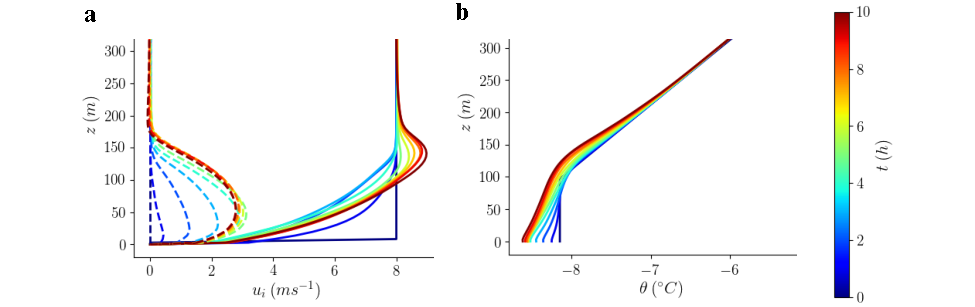
\includegraphics[width=15cm]{figA1.pdf}
\caption{Results of the atmospheric stable boundary layer test case presented in Abkar and Moin (2017) using PALM with the Anisotropic Minimum Dissipation (AMD) turbulence closure. Compare with their Figure 1.} 
\label{fig:validation}
\end{figure*}

\begin{figure*}[t]
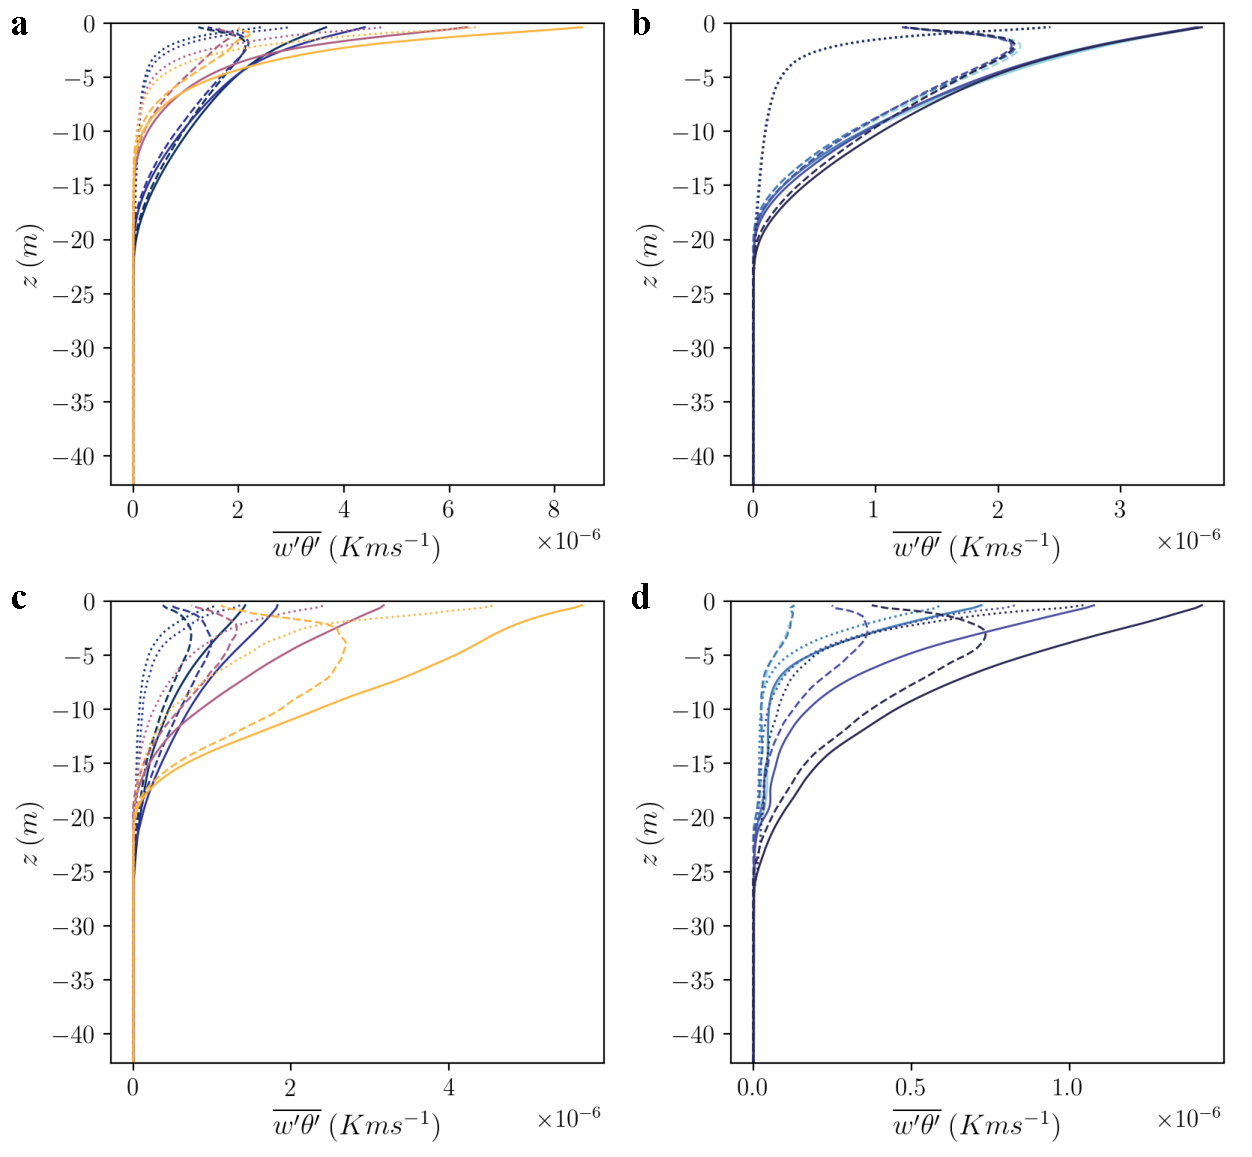
\includegraphics[width=12cm]{figS1.pdf}
\caption{Vertical heat flux depth-profiles averaged over one inertial period for (a,c) thermal driving simulations and (b,d) variable slope simulations. Profiles shown in (a,b) are averaged over the first inertial period after a 2\,\unit{h} spin-up, (b,d) over the last inertial period. Solid lines
represent the total flux, dashed resolved flux and dotted subgrid flux. Colors correspond to those shown in Figure 1.}
\label{fig:res_sgs_flux}
\end{figure*}

\begin{figure}[t]
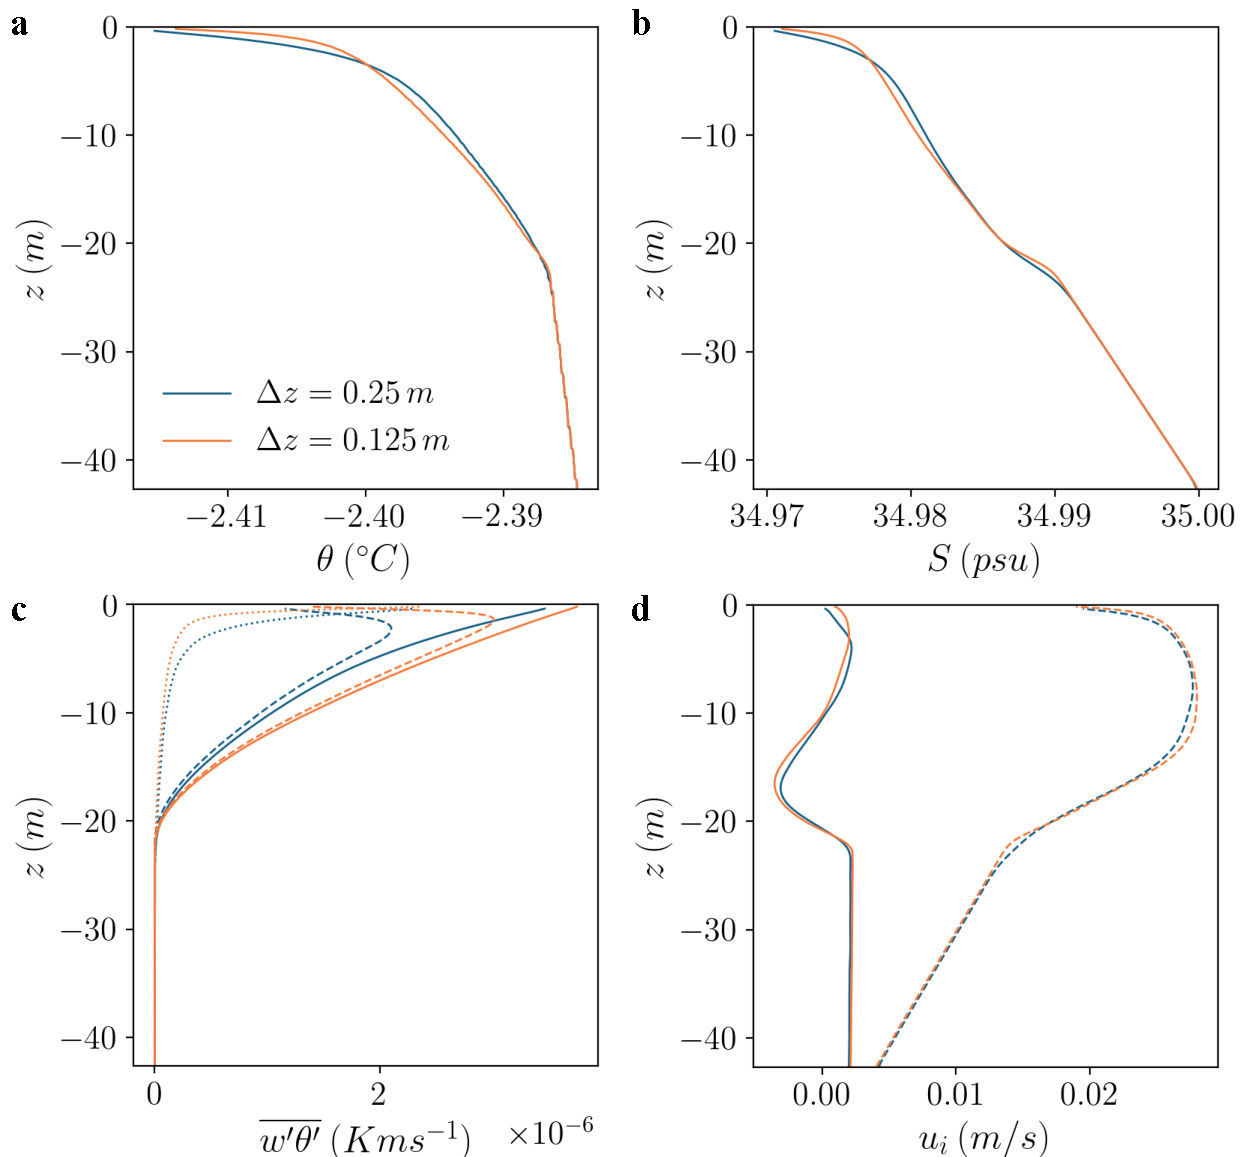
\includegraphics[width=12cm]{figS8.pdf}
\caption{Sensitivity of simulated mean state and turbulent fluxes to resolution. The vertical resolution is double the horizontal resolution ($\Delta x, \Delta y$). Results are averaged over the first inertial period after a 2\unit{h} spin-up. (a) Temperature. (b) Salinity. (c) Total vertical heat flux (solid), resolved vertical heat flux (dashed), and sub-grid vertical heat flux (dotted). (d) Velocity, u-component (solid) and v-component (dashed).}
\label{fig:res_sensitivity}
\end{figure}

\begin{figure*}[t]
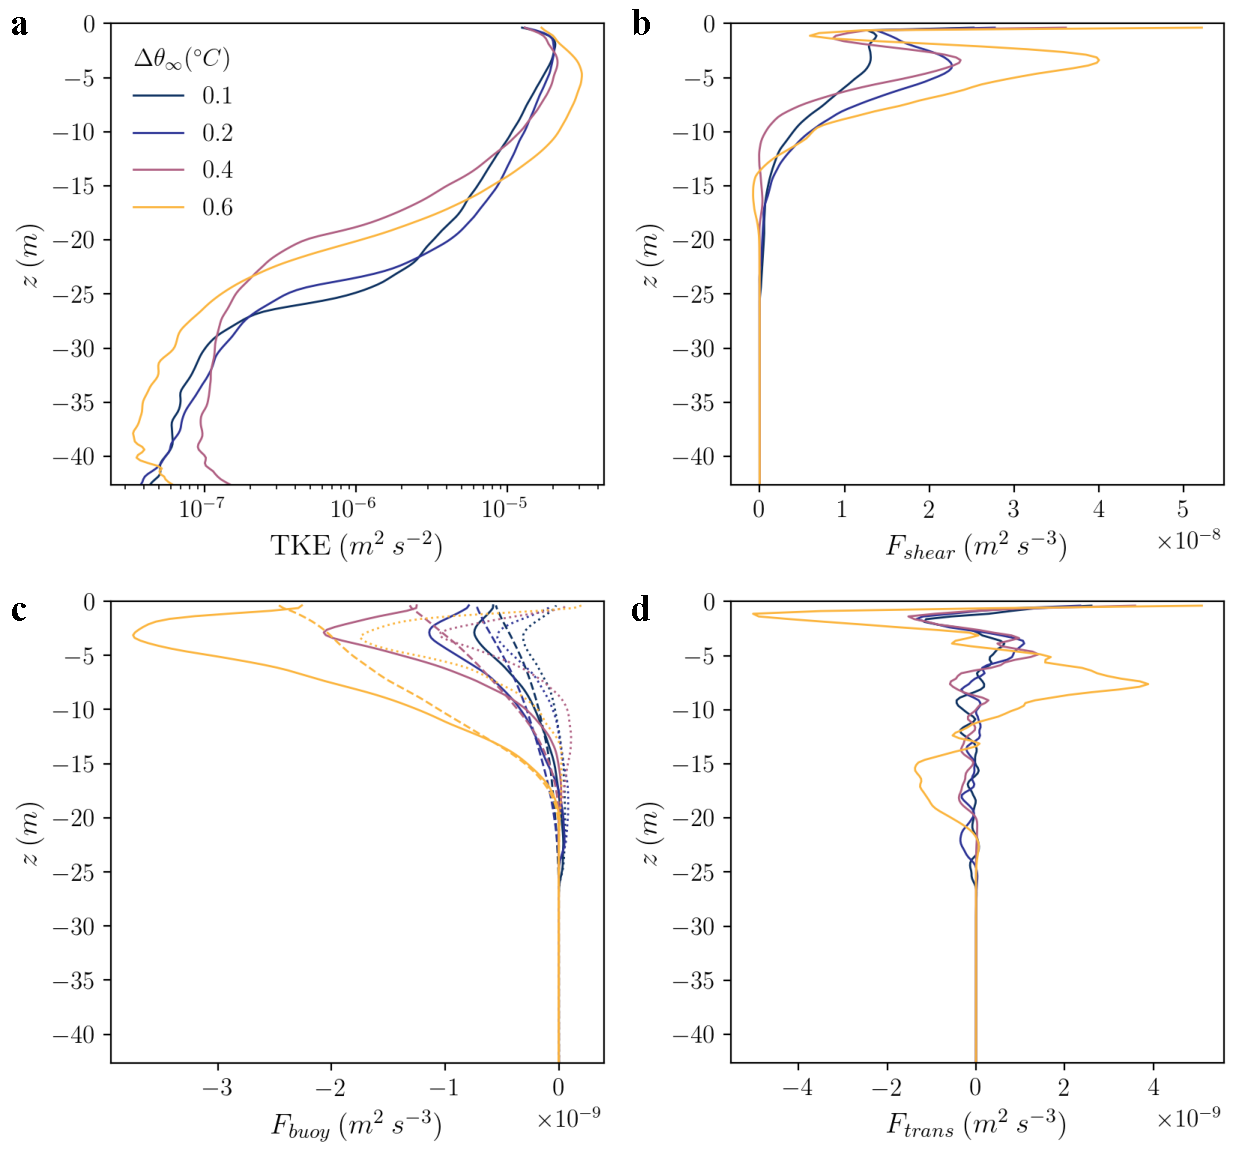
\includegraphics[width=12cm]{figS2.pdf}
\caption{(a) Simulated turbulent kinetic energy for variable thermal driving simulations averaged over the last inertial period and (b-d) turbulent kinetic energy production terms over the same period. (b) Shear production. (c) Buoyancy production. The total buoyancy production is shown with solid lines, vertical component dashed, and upslope component dotted. (d) TKE transport. Positive denotes production, negative destruction. Note that the x-axis scales differ between panels.}
\label{fig:tke_budget_1}
\end{figure*}

\begin{figure*}[t]
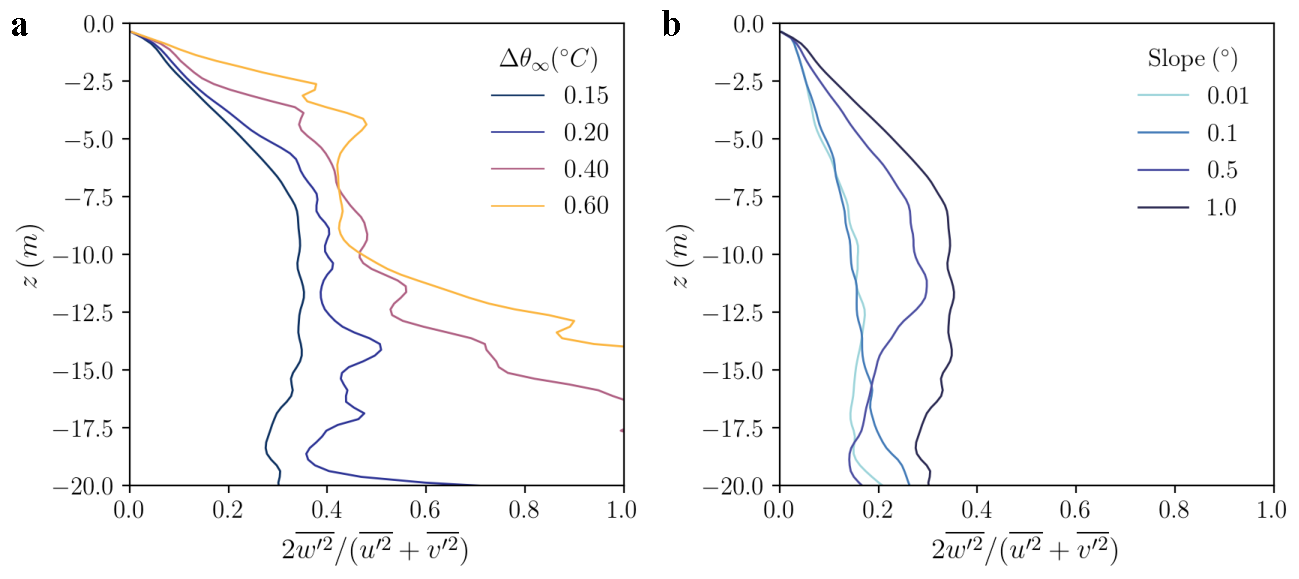
\includegraphics[width=12cm]{figS3.pdf}
\caption{Ratio of vertical to horizontal velocity variance for (a) thermal driving simulations and (b) variable slope simulations averaged over the last inertial period.}
\label{fig:vel_var_ratio}
\end{figure*}

\begin{figure*}[t]
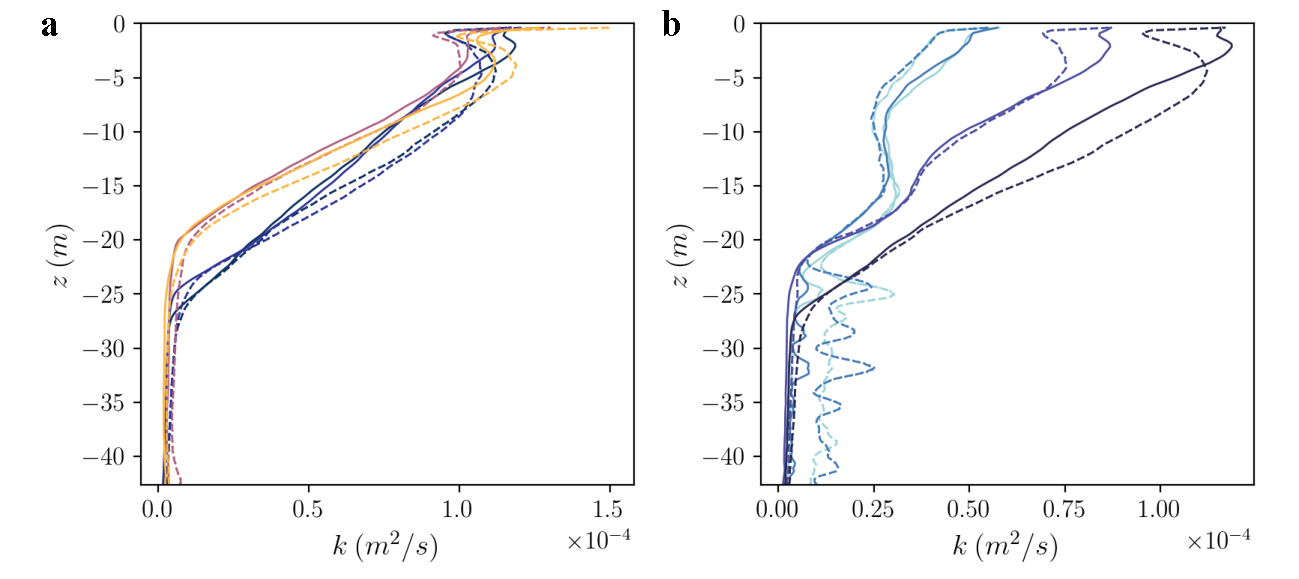
\includegraphics[width=12cm]{figS4.pdf}
\caption{Sub-grid vertical diffusivities for momentum (solid), heat (dashed) and salt (dotted) for (a) thermal driving simulations and (b) variable slope simulations. Heat and salt diffusivities curves are visually indistinguishable.}
\label{fig:k_all}
\end{figure*}

\begin{figure*}[t]
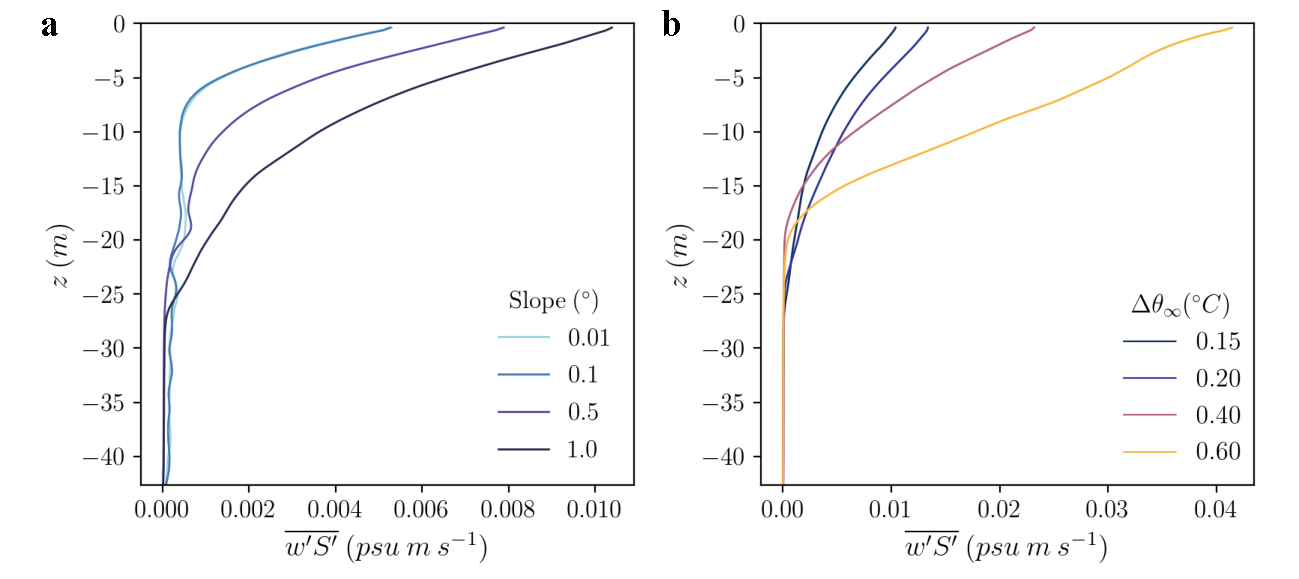
\includegraphics[width=12cm]{figS5.pdf}
\caption{Total vertical salt flux depth-profiles averaged over one inertial period for (a) thermal driving simulations and (b) variable slope simulations.}
\label{fig:saltflux}
\end{figure*}%

\begin{figure*}[t]
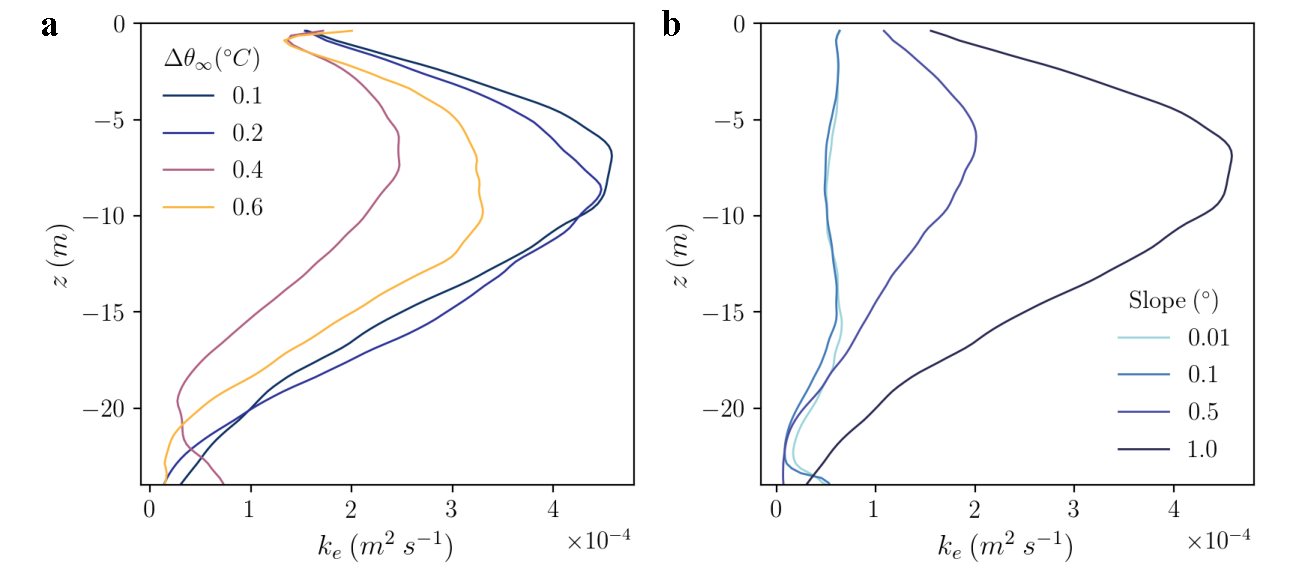
\includegraphics[width=12cm]{figS6.pdf}
\caption{Vertical eddy viscosity from (a) thermal driving simulations and (b) slope-varying simulations over the last inertial period. Depths below -20 m are not shown as the eddy viscosity is only used to compute the Ekman depth within the IOBL. }
\label{fig:km}
\end{figure*}

\begin{figure}[t]
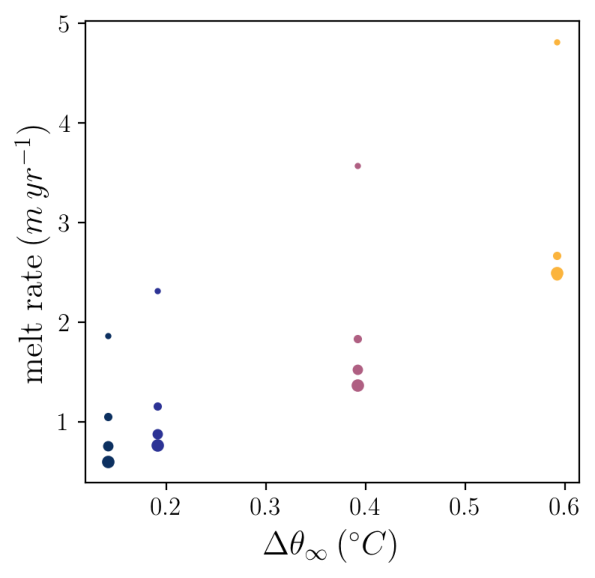
\includegraphics[width=6cm]{figS7.pdf}
\caption{Relationship between far-field thermal driving and melt rate. This figure is the same as Figure 7a but values are averaged over each inertial cycle. The largest points correspond to the fourth and last inertial cycle with progressively smaller points for previous inertial cycles.}
\label{fig:melt_sensitivity_cycles}
\end{figure}

\end{document}